% Chapter 1

\chapter{Introducción General} % Main chapter title

\label{Chapter1} % For referencing the chapter elsewhere, use \ref{Chapter1} 
\label{IntroGeneral}

%----------------------------------------------------------------------------------------

% Define some commands to keep the formatting separated from the content 
\newcommand{\keyword}[1]{\textbf{#1}}
\newcommand{\tabhead}[1]{\textbf{#1}}
\newcommand{\code}[1]{\texttt{#1}}
\newcommand{\file}[1]{\texttt{\bfseries#1}}
\newcommand{\option}[1]{\texttt{\itshape#1}}
\newcommand{\grados}{$^{\circ}$}

%----------------------------------------------------------------------------------------

%\section{Introducción}

En la presente memoria se documenta el trabajo final de la Carrera de Especialización en Sistemas Embebidos que consiste en implementar un \textit{web server} utilizando la plataforma CIAA-NXP, el RTOS freeRTOS V8.0.1, y el stack TCP/IP lwip V1.41. 

Se busca satisfacer una necesidad relacionada con los acuarios. En particular, interesa poder controlar un número de variables indicativas del estado del mismo.  Se busca implementar una interfaz web que permita visualizar información relevante sobre el estado del acuario y permita actuar sobre las variables cuyas desviaciones respecto a valores de referencia, pueden afectar negativamente al entorno.  Asimismo, se busca facilitar tareas de mantenimiento que se deben realizar en forma rutinaria y que son de vital importancia para la supervivencia de los seres vivos que habitan en el acuario, principalmente peces, invertebrados y plantas. Detalles referentes a qué son los acuarios serán abordados en la sección \ref{sec:acuario}.

Se implementa un firmware de monitoreo y control sobre una de las plataformas de hardware desarrollada por el Proyecto Computadora Industrial Abierta Argentina, denominado de ahora en adelante Proyecto-CIAA, en particular la versión CIAA-NXP que utiliza un microprocesador fabricado por la empresa NXP. El Proyecto-CIAA se trata en la sección \ref{sec:proyecto-ciaa}.

Debido a la vasta difusión de las redes de computadoras y la tendencia mundial a incorporar cada día más dispositivos a internet, fenómeno también conocido con el internet de las cosas o IoT (por sus siglas en inglés \textit{Internet of Things}) se opta por desarrollar una interfaz web embebida en la CIAA-NXP.  Dicha interfaz es accesible mediante el protocolo ethernet a través de una red de área local o LAN (por sus siglas en inglés \textit{Local Area Network}). Detalles de la implementación se abordan en la sección \ref{sec:interfaz-web}.

\clearpage
\section{¿Qué es el Proyecto CIAA?}
\label{sec:proyecto-ciaa}

El Proyecto CIAA (Computadora Industrial Abierta Argentina) nació en 2013 como una iniciativa conjunta entre el sector académico y el industrial, representados por la ACSE\footnote{Asociación Civil para la investigación, promoción y desarrollo de los Sistemas electrónicos Embebidos.} y CADIEEL\footnote{Cámara Argentina de Industrias Electrónicas, Electromecánicas y Luminotécnicas.}, respectivamente \citep{CIAA}.

% Sitio web: \url{http://www.sase.com.ar/asociacion-civil-sistemas-embebidos}
% Sitio web: \url{http://www.cadieel.org.ar/}
%ACSE\footnote{\url{http://www.sase.com.ar/asociacion-civil-sistemas-embebidos}} y CADIEEL\footnote{\url{http://www.cadieel.org.ar}}, respectivamente. 

Objetivos del proyecto:

\begin{itemize}
	\item Impulsar el desarrollo tecnológico nacional, a partir de sumar valor agregado al trabajo y a los productos y servicios, mediante el uso de sistemas electrónicos, en el marco de la vinculación de las instituciones educativas y el sistema científico-tecnológico con la industria.
	\item Darle visibilidad positiva a la electrónica argentina.
	\item Generar cambios estructurales en la forma en la que se desarrollan y utilizan en nuestro país los conocimientos en el ámbito de la electrónica y de las instituciones y empresas que hacen uso de ella.
\end{itemize}

Todo esto en el marco de un trabajo libre, colaborativo y articulado entre industria y academia. 

En el marco de esta iniciativa se han desarrollado distintas plataformas de \textit{hardware}, un \textit{firmware} con drivers y ejemplo de aplicación y un entorno de desarrollo basado en el \textit{software} eclipse.

Dentro de las plataformas de \textit{hardware} se encuentran versiones basadas en distintos microcontroladores de distintos fabricantes y versiones sobre FPGA (\textit{Field Programmable Gate Array}).  También hay versiones pensadas para trabajar en ambientes industriales y versiones educativas que utilizan el mismo microcontrolador pero a un costo total menor que la versión industrial. 
A continuación se listan las plataformas que se encuentra en fase de comercialización.

\begin{itemize}
\item CIAA-NXP, primera plataforma industrial desarrollada por el proyecto.  Se basa en el microcontrolador NXP LPC4337. 
%\vspace{5px
\item EDU-CIAA-NXP, versión de bajo costo de la CIAA-NXP pensada para la enseñanza universitaria, terciaria y secundaria. 
\end{itemize}

Asimismo, existen otras versiones en desarrollo, CIAA-FSL, EDU-CIAA-FSL, CIAA-Safety, CIAA-ACC, EDU-CIAA-XILINX, EDU-CIAA-INTEL y CIAA-PIC. Información detallada respecto a cada plataforma y su grado de avance se puede encontrar en \citep{CIAA}.

%\begin{itemize}
%\item CIAA-FSL, basada en el microcontrolador Freescale MK60FX512VLQ15.
%%\vspace{5px}
%\item EDU-CIAA-FSL es una versión de bajo costo de la CIAA-FSL pensada para la enseñanza universitaria, terciaria y secundaria.
%%\vspace{5px}
%\item CIAA-Safety, para aplicaciones que requieran de Seguridad Funcional Certificable bajo norma IEC 61508. Basada en el microcontrolador TI RM48L952.
%%\vspace{5px}
%\item CIAA-ACC para aplicaciones de Alto Costo Computacional. Basada en tecnología FPGA.
%%\vspace{5px}
%\item EDU-CIAA-XILINX es una plataforma de bajo costo para el aprendizaje de los sistemas embebidos implementados con softcores sobre FPGA.
%%\vspace{5px}
%\item EDU-CIAA-INTEL es una plataforma de desarrollo de bajo costo basada en el SoM Edison de Intel.
%%\vspace{5px}
%\item CIAA-PIC, basada en el microcontrolador Microchip PIC32MZ2048ECH144.
%\end{itemize}

Debido a que el trabajo requiere una plataforma totalmente desarrollada y conexión ethernet, se elige la plataforma industrial CIAA-NXP. Se detallan en la sección \ref{sec:ciaa-nxp} las principales características de la misma.

\subsection{Plataforma CIAA-NXP}
\label{sec:ciaa-nxp}

La CIAA-NXP es la primera y única computadora del mundo que reúne dos cualidades:

\begin{itemize}
\item 
Ser \textbf{Industrial}, ya que su diseño está preparado para las exigencias de confiabilidad, temperatura, vibraciones, ruido electromagnético, tensiones, cortocircuitos, etc., que demandan los productos y procesos industriales.
\item 
Ser \textbf{Abierta}, ya que toda la información sobre su diseño de hardware, firmware, software, etc. está libremente disponible en Internet bajo la Licencia BSD, para que cualquiera la utilice como quiera.
\end{itemize}

\begin{figure}[h!]
	\centering
    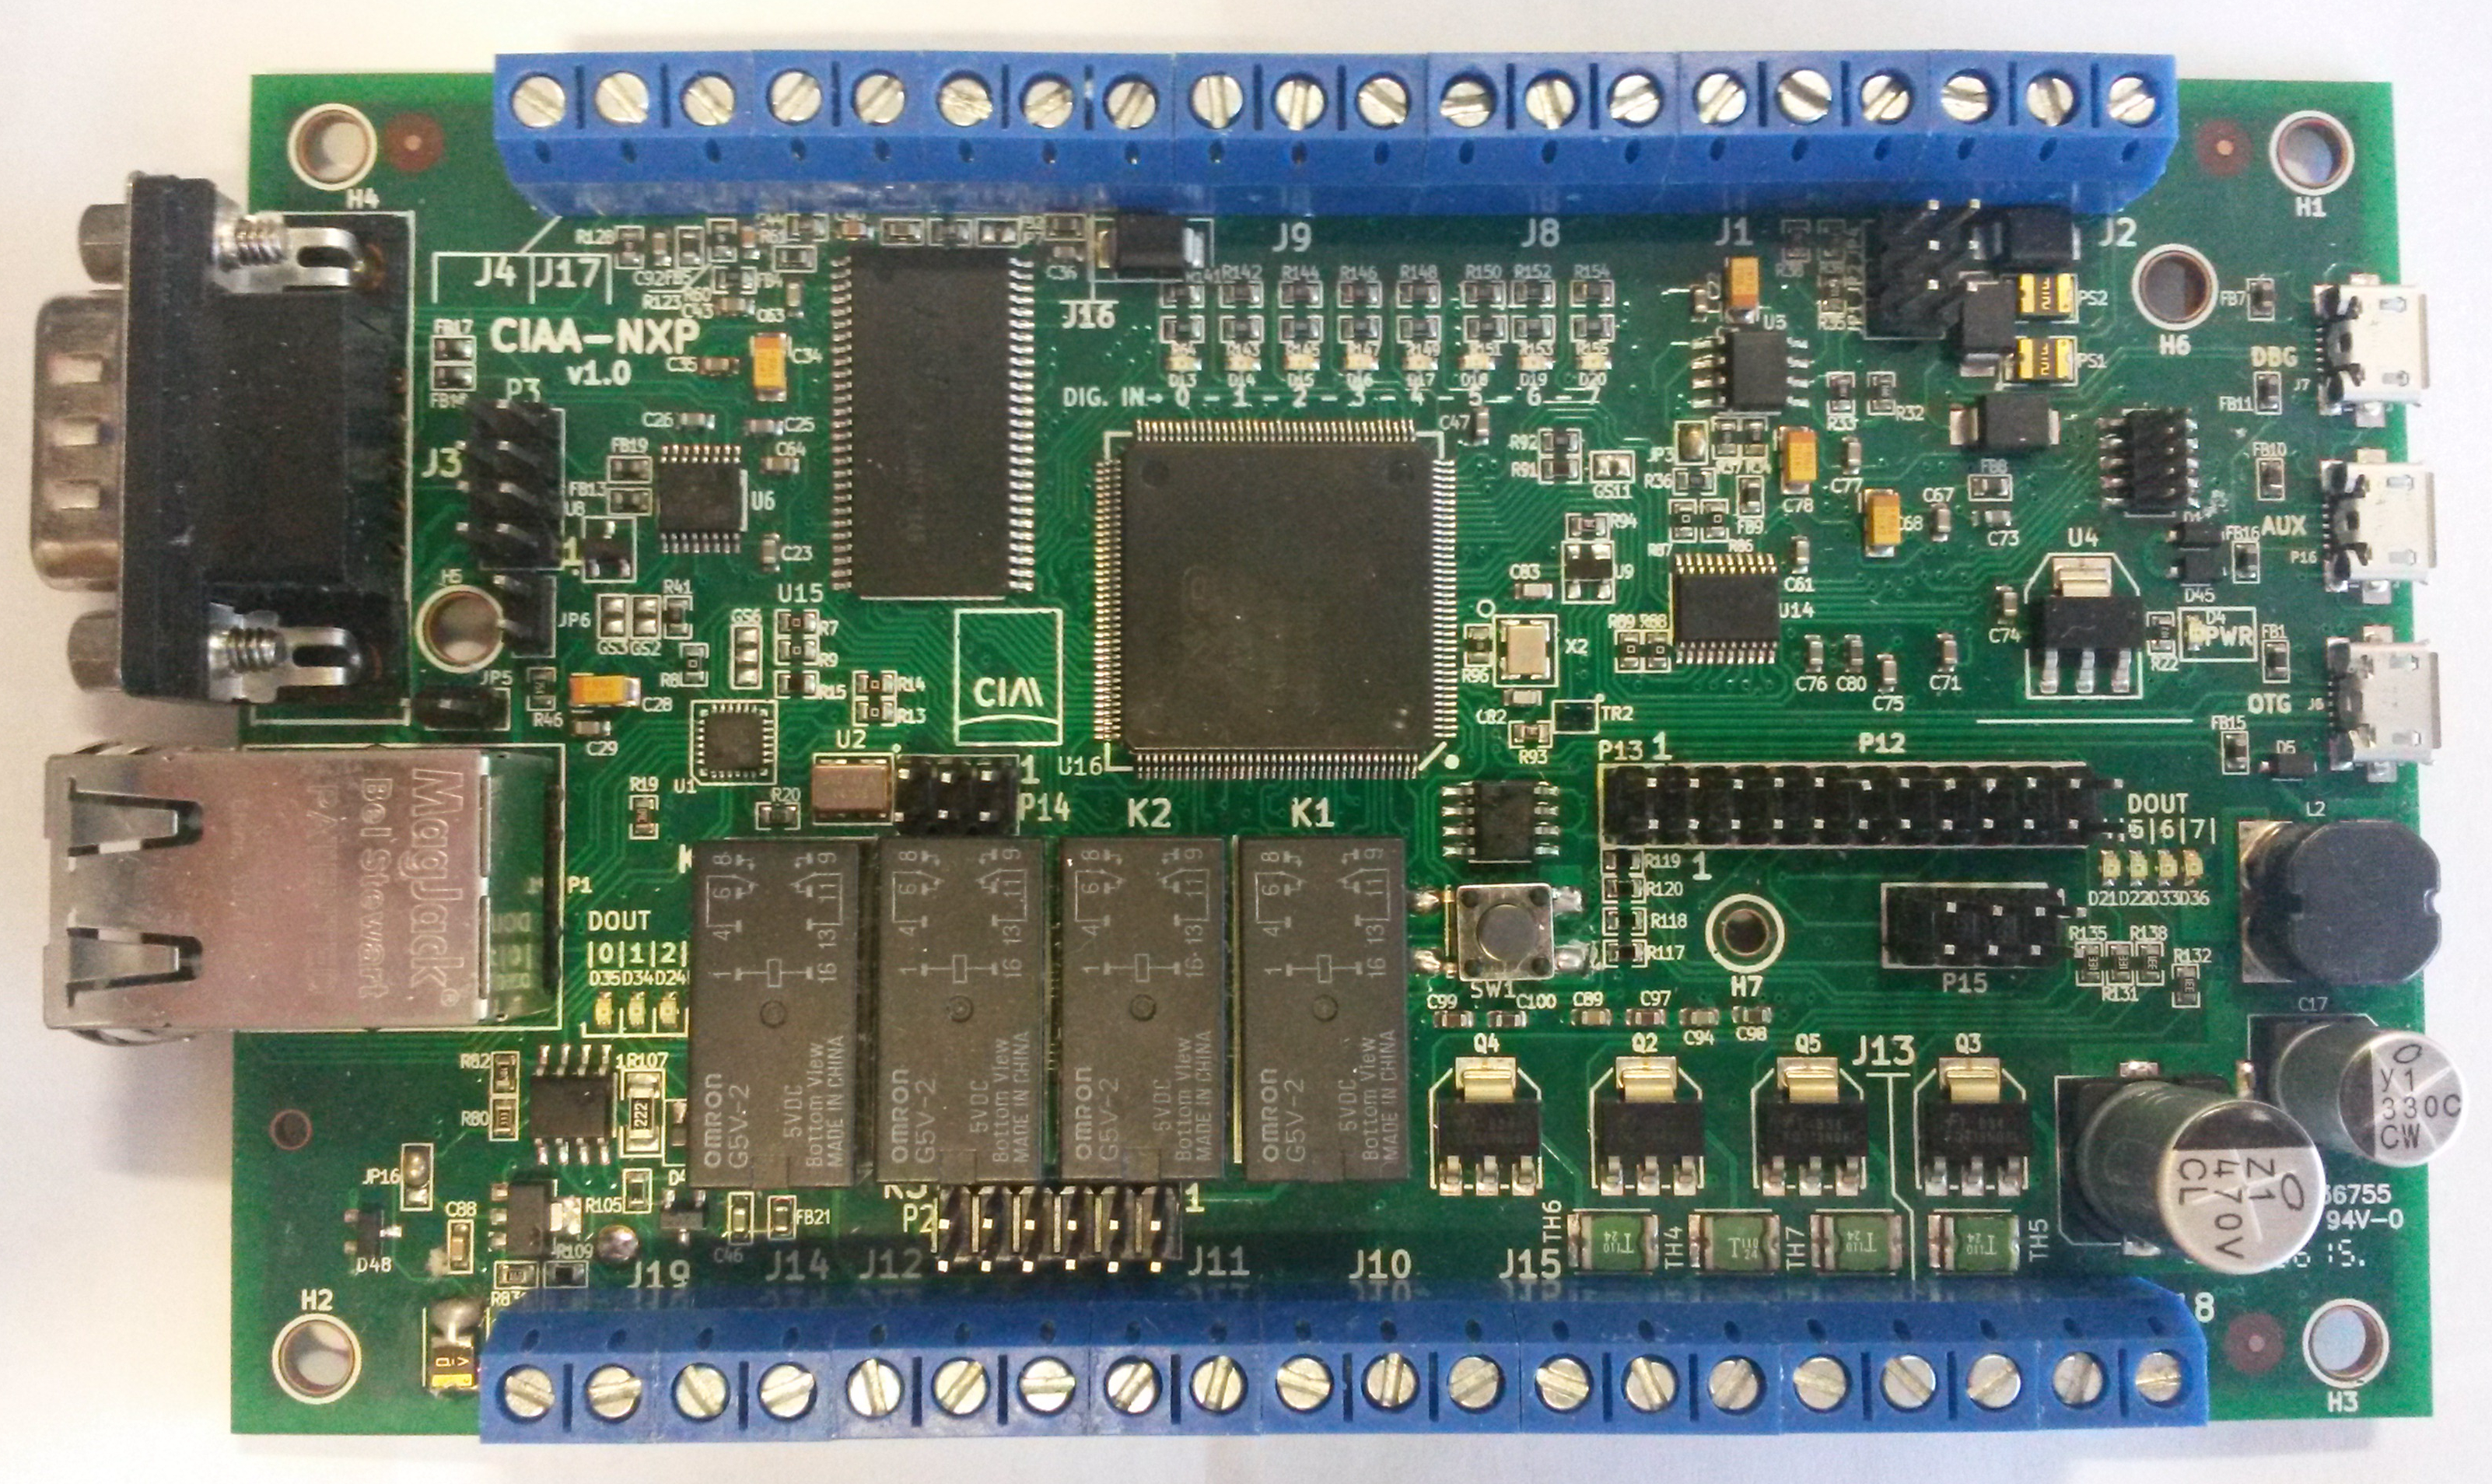
\includegraphics[width=.8\textwidth]{./Figures/ciaa-nxp.jpg}
	\label{fig:ciaa-nxp}
	\caption{Plataforma CIAA-NXP}
\end{figure}


\noindent Esta plataforma se compone de:

\begin{itemize}
\item CPU: Microcontrolador NXP LPC4337JBD144 (Dual-core Cortex-M4 + Cortex-M0 @ 204MHz).
\item Debugger: USB-to-JTAG FT2232H. Soportado por OpenOCD.
\item Memorias: 
   \begin{itemize}
   \item IS42S16400F - SDRAM. 64Mbit @ 143MHz.
   \item S25FL032P0XMFI011 - Flash SPI. 32 Mbit, Quad I/O Fast read: 80 MHz.
   \item 24AA1025 - EEPROM I2C. 1 Mbit, 400 kHz. Almacenamiento de propósito general, datos de calibración del usuario, etc.
   \item 24AA025E48 - EEPROM I2C. 2 kbit, 400 kHz. Para implementación de MAC-Address o almacenamiento de propósito general.
   \end{itemize}
\item Entradas y salidas:   
   \begin{itemize}
   \item 8 entradas digitales opto-acopladas.
   \item 4 entradas analógicas 0-10V/4-20mA.
   \item 4 salidas Open-Drain. 
   \item 4 salidas con Relay DPDT.
   \item 1 salida analógica 0-10V/4-20mA.
   \end{itemize}
\item LV-GPIO:
   \begin{itemize}
   \item 14 GPIOs.
   \item I2C.
   \item SPI.
   \item 4 canales analógicos.
   \item Aux. USB.
   \end{itemize}
\item
Interfaces de comunicación:
   \begin{itemize}
   \item Ethernet.
   \item USB On-The-Go.
   \item RS232.
   \item RS485.
   \item CAN.
   \end{itemize}
\item Múltiples fuentes de alimentación.

\end{itemize}

\section{¿Qué es un Acuario?}
\label{sec:acuario}

El Acuarismo es una actividad comercial y recreativa ampliamente difundida en la Argentina que consiste en establecer y mantener un ecosistema acuático artificial. El término acuario o pecera se utiliza indistintamente para referirse tanto al contenedor de agua como a todo el ecosistema artificial. 

Un acuario puede albergar a un número determinado de peces, plantas e invertebrados y para su mantenimiento es preciso recrear un biotopo\footnote{Territorio o espacio vital cuyas condiciones ambientales son las adecuadas para que en él se desarrolle una determinada comunidad de seres vivos.} en función de los hábitos y costumbres de las especies que lo habiten; a modo de ejemplo, existen vertebrados acuáticos aptos para vivir en agua fría, otros requieren un sistema calefactor para mantener el agua en un microclima cálido, incluso las especies marinas precisan cuidados más específicos en cuanto al tratamiento del agua.

Los acuarios se clasifican principalmente según las condiciones del agua:
\begin{itemize}
	\item Por temperatura
	\begin{itemize}
		\item Agua fría; entorno a los 18 \grados C.
		\item Agua tropical; normalmente entre 22 y 27 \grados C.
	\end{itemize}
	\vspace{5px}
	\item Por salinidad
	\begin{itemize}
		\item Agua dulce; baja concentración de sales disueltas.
		\item Salobre; agua con entre 0.5 y 30 gr. de sal por litro.
		\item Agua de mar o Marinos; 35 gr. de sal por litro. 
	\end{itemize}
\end{itemize}

El punto de entrada recomendado para principiantes en la disciplina es el acuario de agua dulce y fría de al menos 90 litros.  Su mantenimiento es más sencillo que el de los acuarios marinos y los peces de agua fría son los más resistentes y los que presentan mayor compatibilidad entre especies. Normalmente se pueden mantener con agua de red debidamente declorada y acondicionada. Finalmente, un acuario más grande es más fácil de mantener, sobre todo en lo referido al tratamiento del agua y a conseguir una temperatura estable para los peces \citep{paradais1}.

\subsection{Parámetros del agua}

A través del agua los peces, plantas y bacterias que habitan el acuario incorporan nutrientes y eliminan desechos. Entre ellos se conformar una cadena biológica con interacciones complejas. Los desechos de unos son aprovechados como nutrientes de otros.  A modo de ejemplo se puede mencionar como las colonias de microorganismos (básicamente bacterias), en etapas diferenciadas, pueden ``procesar'' los compuestos orgánicos contaminantes provenientes de los peces, y transformarlos en compuestos inofensivos o que puedan ser integrados en los tejidos de algas y plantas del acuario. \citep{teton2003}


Es necesario que el agua se encuentre debidamente tratada de acuerdo con las necesidades específicas que requiera la especie de peces que se pretenda albergar.  Asimismo, se debe asegurar la mayor estabilidad de las condiciones del agua posibles ya que los seres vivos que en ella habitan son sensibles a las variaciones bruscas.  Se deben tener en cuenta los siguientes parámetros del agua:

\begin{itemize}
		\item La Dureza es una medida de la cantidad de sales minerales, particularmente las sales de calcio y magnesio que se encuentran disueltas.
		\item Concentración CO2  o anhídrido carbónico.
		\item El valor pH refiere a la cantidad de iones libres de hidrógeno. Refleja el carácter ácido o alcalino del medio. El pH viene establecido por dos componentes, la dureza de carbonatos y el CO2. La relación entre ambos, la dureza de carbonatos como el componente alcalino y el CO2 como componente ácido, son los que establecen el valor del PH. Si la relación es similar el PH es neutro, cercano al valor 7.
		\item Concentración CO2  o anhídrido carbónico.
		\item La salinidad, representa la masa total de sales (en mg) disueltos por litro de agua.
\end{itemize}


Los peces viven bien con un pH que oscile entre 5 y 9, con valores extremos, tanto hacia el 0 como hacia el 14, sólo son aptos peces muy especializados.

Por lo general el pH más correcto para el pleno desarrollo de los peces es el que se encuentra entre 5.5 y 7.5. Hay que tener en cuenta que lo ideal, o sea, la neutralidad es 7.

%
%\begin{figure}[]
%	\centering
%    \includegraphics[width=.5\textwidth]{./Figures/acuarioHobby3.jpg}
%	\label{fig:acuarioHobby}
%	\caption{Acuario de un individuo particular}
%\end{figure}       
%
%\begin{figure}[]
%	\centering
%    \includegraphics[width=.7\textwidth]{./Figures/acuarioTienda.jpg}
%	\label{fig:acuarioTienda}
%	\caption{Tienda de insumos para Acuario}
%\end{figure}


%----------------------------------------------------------------------------------------

\section{Motivación}

Según el tipo de actividad se pueden encontrar acuarios con fines productivos para la recreación de especies destinadas al consumo humano.  Por otra parte

De conversaciones con personas que practican el acuarismo se tomó conocimiento de la existencia de una necesidad no satisfecha de un equipo electrónico que permita controlar las variables de estado de un acuario. 
 
Las personas consultadas manifestaron no conocer equipos que puedan realizar estas u otras funciones más complejas y que se comercialicen en el mercado local.  

Asimismo, se consultaron distintas locales de venta de insumos para acuarios de capital federal vía e-mail preguntando si tenían a la venta o conocían la existencia de un equipo para satisfacer la necesidad planteada y la respuesta fue abrumadoramente negativa. Como se detallará en la sección \ref{sec:existentes}, existen soluciones comerciales disponibles pero no se comercializan en el mercado local, lo cuál permite afirmar que la necesidad planteada no esta debidamente satisfecha y existe un mercado potencial que se analizará en la sección \ref{sec:mercado}.
%
%\begin{figure}[h!]
%	\centering
%    \includegraphics[width=.9\textwidth]{./Figures/nemo.jpg}
%	\label{fig:nemo}
%	\caption{Pez payaso}
%\end{figure}

\subsection{Dimensionamiento del mercado}
\label{sec:mercado}

\subsection{Soluciones existentes}
\label{sec:existentes}

%\begin{minipage}[c]{1.0\linewidth}
%\begin{minipage}[c]{0.6\linewidth}
%	\begin{itemize}
%		\item Ecosistema vivo y dinámico 
%		% Recreación de un ambiente subacuático para albergar peces, invertebrados y plantas
%		\vspace{10px}
%		\item Interacciones complejas
%		\vspace{10px}
%		\item Uso recreativo o comercial
%		\vspace{10px}
%		\item Malas condiciones = \$
%		\vspace{10px}
%  	\end{itemize}	
%  \end{minipage}
%  \begin{minipage}[c]{0.35\linewidth}
%	\begin{figure}[H]
%		{\includegraphics[width=1\textwidth]{./imagenes/acuario.jpg}}
%	\end{figure}	  	  	
%  \end{minipage}
%\end{minipage}
%\end{frame}

%\begin{figure}[h!]
%	\centering
%    \includegraphics[width=.5\textwidth]{./Figures/profilux}
%	\label{fig:competencia1}
%	\caption{Solución existente 1}
%\end{figure}
%
%\begin{figure}[h!]
%	\centering
%    \includegraphics[width=.5\textwidth]{./Figures/reefkeeper}
%	\label{fig:competencia2}
%	\caption{Solución existente 2}
%%	\footnote{Referencia a la figura}
%\end{figure}


\subsection{Aplicabilidad a otras áreas}





%----------------------------------------------------------------------------------------
